\documentclass[tikz]{standalone}
\usetikzlibrary{shapes.geometric}
\usepackage{tikz}
\usepackage{standalone}
\begin{document}
	
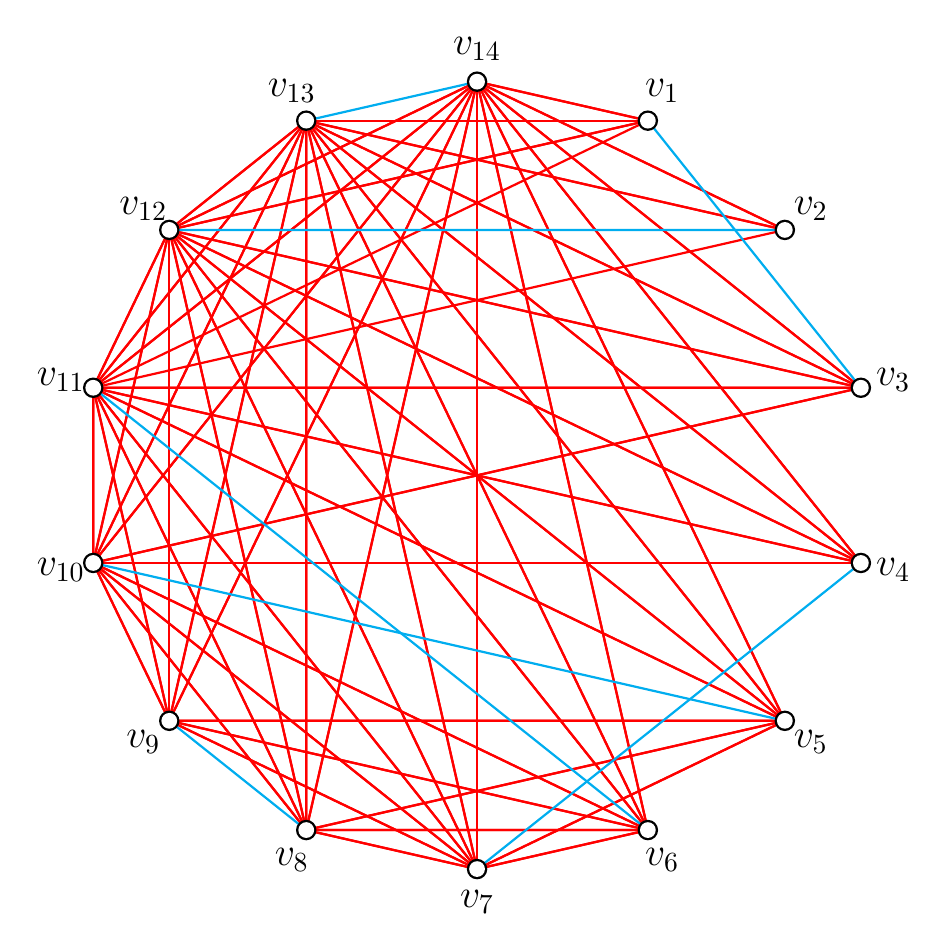
\begin{tikzpicture}
%Values of nodes:
% 0 = 1
% 1 = 1
% 2 = 2
% 3 = 2
% 4 = 3
% 5 = 3
% 6 = 4
% 7 = 4
% 8 = 4
% 9 = 5
% 10 = 6
% 11 = 7
% 12 = 7
% 13 = 7
% threshold tau = 7

%\foreach \n in {0,...,13}
\foreach \n in {1,...,14}
	\fill (90-\n*25.71428571:5cm) coordinate (v\n) circle [radius = 0.1]
		++(90-\n*25.71428571:12pt) node {\Large{$v_{\n}$}};
\foreach \m/\n in {1/12,1/13,1/14,2/13,2/14,3/10,3/11,3/12,3/13,3/14,4/10,4/11,4/12,4/13,4/14,5/7,5/8,5/9,5/11,5/12,5/13,5/14,6/7,6/8,6/9,6/10,6/12,6/13,6/14,7/5,7/6,7/8,7/9,7/10,7/11,7/12,7/13,7/14,8/5,8/6,8/7,8/10,8/11,8/12,8/13,8/14,9/5,9/6,9/7,9/10,9/11,9/12,9/13,9/14,10/3,10/4,10/6,10/7,10/8,10/9,10/11,10/12,10/13,10/14,11/1,11/2,11/3,11/4,11/5,11/7,11/8,11/9,11/10,11/12,11/13,11/14,12/1,12/3,12/4,12/5,12/6,12/7,12/8,12/9,12/10,12/11,12/13,12/14,13/1,13/2,13/3,13/4,13/5,13/6,13/7,13/8,13/9,13/10,13/11,13/12,14/1,14/2,14/3,14/4,14/5,14/6,14/7,14/8,14/9,14/10,14/11,14/12}
%{0/11,0/12,0/13,1/12,1/13,2/9,2/10,2/11,2/12,2/13,3/9,3/10,3/11,3/12,3/13,4/6,4/7,4/8,4/10,4/11,4/12,4/13,5/6,5/7,5/8,5/9,5/11,5/12,5/13,6/4,6/5,6/7,6/8,6/9,6/10,6/11,6/12,6/13,7/4,7/5,7/6,7/9,7/10,7/11,7/12,7/13,8/4,8/5,8/6,8/9,8/10,8/11,8/12,8/13,9/2,9/3,9/5,9/6,9/7,9/8,9/10,9/11,9/12,9/13,10/0,10/1,10/2,10/3,10/4,10/6,10/7,10/8,10/9,10/11,10/12,10/13,11/0,11/2,11/3,11/4,11/5,11/6,11/7,11/8,11/9,11/10,11/12,11/13,12/0,12/1,12/2,12/3,12/4,12/5,12/6,12/7,12/8,12/9,12/10,12/11,13/0,13/1,13/2,13/3,13/4,13/5,13/6,13/7,13/8,13/9,13/10,13/11}
	\draw [thick, red] (v\n) -- (v\m);
%\foreach \m/\n in {0/2, 1/11, 3/6, 4/9, 5/10, 7/8, 12/13}
\foreach \m/\n in {1/3, 2/12, 4/7, 5/10, 6/11, 8/9, 13/14}
	\draw [thick, cyan] (v\n) -- (v\m);
%\foreach \n in {0,...,13}
\foreach \n in {1,...,14}
	\fill (90-\n*25.71428571:5cm) coordinate (v\n) circle [radius = 0.13];
%\foreach \n in {0,...,13}
\foreach \n in {1,...,14}
	\fill [white] (90-\n*25.71428571:5cm) coordinate (v\n) circle [radius = 0.1];

\end{tikzpicture}
	
\end{document}